%=====================================================================
% Open Science Journal — Draft Manuscript
% Coupled flood–seismicity multi-hazard test bed
%=====================================================================

\documentclass[12pt, a4paper]{article}

\usepackage[utf8]{inputenc}
\usepackage[T1]{fontenc}
\usepackage{times}
\usepackage{setspace}
\usepackage{lineno}
\usepackage{geometry}
\usepackage{graphicx}
\usepackage{booktabs}
\usepackage{amsmath, amssymb, amsthm}
\usepackage{mathtools}
\usepackage{url}
\usepackage[hidelinks]{hyperref}
\usepackage{enumitem}
\usepackage{caption}
\usepackage{float}
\usepackage{verbatim}
\usepackage{listings}

\geometry{top=2.5cm, bottom=2.5cm, left=2.5cm, right=2.5cm}
\doublespacing
\renewcommand{\footnote}[1]{}

\theoremstyle{plain}
\newtheorem{proposition}{Proposition}
\newtheorem{corollary}{Corollary}
\theoremstyle{definition}
\newtheorem{definition}{Definition}
\theoremstyle{remark}
\newtheorem{remark}{Remark}

\newcommand{\keywords}[1]{\vspace{0.5em}\noindent\textbf{Keywords:} #1}
\newcommand{\R}{\mathbb{R}}
\newcommand{\bx}{\mathbf{x}}
\newcommand{\bF}{\mathbf{F}}
\newcommand{\bk}{\mathbf{k}}
\newcommand{\bI}{\mathbf{I}}
\newcommand{\bP}{\mathbf{P}}
\newcommand{\bA}{\mathbf{A}}
\newcommand{\bJ}{\mathbf{J}}
\newcommand{\bS}{\mathbf{S}}
\newcommand{\bM}{\mathbf{M}}
\newcommand{\bL}{\mathbf{L}}

\lstset{
  basicstyle=\ttfamily\small,
  breaklines=true,
  frame=single,
  columns=fullflexible,
  keepspaces=true,
  showstringspaces=false
}

\title{\textbf{Deterministic Permutation Scheduling for Coupled
Flood--Seismicity Models: Unconditional Instability of Full Coupling and a
Period-Two Remedy}}

\author{
  First Author\textsuperscript{1,*},
  Second Author\textsuperscript{2},
  Third Author\textsuperscript{1}
}

\date{
  \textsuperscript{1}Department of Applied Mathematics, University of Example,
  City, Country \\
  \textsuperscript{2}Institute of Computational Science, Example Research
  Centre, City, Country \\
  \textsuperscript{*}Corresponding author: email@example.com
}

\begin{document}
\linenumbers
\maketitle

%---------------------------------------------------------------------
\begin{abstract}
\noindent
Multi-hazard early-warning systems that couple hydrological and seismic
subsystems must reconcile two data streams that arrive asynchronously. A
natural modelling device is to let a pre-recorded binary schedule decide, at
each step, which coupling direction is active, with the exchange represented
by a permutation matrix. We formalise this device, define an exact coupling
coefficient, and show that its stability properties are not governed by that
coefficient. For a two-block linearisation representative of a
reservoir--fault system, the fully coupled schedule is unstable for every
step size, while a period-two alternating schedule with half the nominal
coupling recovers the classical uncoupled bound. We give the closed-form
two-step monodromy matrix and report spectral radii verified at five step
sizes. A stylized flood--seismicity test bed and runnable code accompany the
analysis. The practical conclusion is that coupling strength alone does not
determine stability, and that the full schedule must be reported.

\keywords{multi-hazard coupling, deterministic scheduling, switched systems,
reservoir-induced seismicity, numerical stability, monodromy matrix}
\end{abstract}

\newpage

%---------------------------------------------------------------------
\section{Introduction}
\label{sec:intro}

Operational multi-hazard platforms increasingly fuse hydrological and seismic
data into a single forecasting pipeline. Reservoir operations, for example,
are monitored alongside local seismicity because filling and drawdown are
known to modulate earthquake occurrence \cite{simpson1976,gupta1992}, and
conversely because ground shaking alters permeability, dam integrity, and
gauge behaviour \cite{scholz1998}. The two subsystems are physically coupled
in both directions, but the coupling is rarely active in both directions at
once. Data arrive on different clocks: water-level gauges report hourly,
seismic networks report event-triggered, and the integration step is often
chosen to match neither.

When the exchange pattern is dictated by a recorded event log rather than by a
random process, the resulting integrator is deterministic but
\emph{state-dependent in structure}. The simplest formalisation is a binary
schedule: at step $k$ a value $s_k \in \{0,1\}$ selects whether the vector
field is evaluated in its natural ordering or in a permuted ordering. The
permutation is fixed and represented by a permutation matrix $\bP$.

This construction sits at the intersection of three literatures. It is a
special case of operator splitting and composition \cite{strang1968,mclachlan2002};
it is a switched or hybrid system in the sense of Liberzon \cite{liberzon2003};
and because permutations are orthogonal, it superficially resembles a
geometric integrator \cite{hairer2006,leimkuhler2004,leimkuhler2004}. We show
that the third resemblance is misleading.

Our contributions are four. First, we give a self-contained formulation and an
exact coupling coefficient (Sections~\ref{sec:formulation}--\ref{sec:coupling}).
Second, we show that the fourth-order Runge--Kutta extension retains its
classical order when the switch is frozen across each step
(Section~\ref{sec:rk}). Third, we prove that for a two-block linearisation the
fully coupled schedule has a positive real eigenvalue in the permuted field
and is therefore unstable for \emph{every} step size, not merely for large
ones (Section~\ref{sec:stability}). Fourth, we show that a period-two
alternating schedule restores a finite stability window and give its
monodromy matrix in closed form. Section~\ref{sec:testbed} sets out a stylized
flood--seismicity test bed, Section~\ref{sec:discussion} discusses scope, and
Section~\ref{sec:conclusions} concludes.

%---------------------------------------------------------------------
\section{Formulation}
\label{sec:formulation}

\subsection{The scheduled explicit Euler map}

Let the state at step $k$ be $\bx_k \in \R^n$, let $h>0$ be the step size, and
let $\bP \in \R^{n\times n}$ be a fixed permutation matrix. Let
$\{s_k\}_{k\ge0} \subset \{0,1\}$ be a deterministic binary schedule supplied
by the user. The scheduled explicit Euler iteration is
\begin{equation}
\bx_{k+1} = \bx_k + h\,\bF^{(s_k)}(\bx_k),
\label{eq:euler}
\end{equation}
with the scheduled field
\begin{equation}
\bF^{(s_k)}(\bx_k) = \bL_{s_k}\bF(\bx_k),
\qquad
\bL_s := (1-s)\bI + s\bP .
\label{eq:field}
\end{equation}
Expanding the operator gives the working form
\begin{equation}
\boxed{\;\bx_{k+1} = \bx_k + h\Big((1-s_k)\,\bF(\bx_k) + s_k\,\bP\bF(\bx_k)\Big).\;}
\label{eq:boxed}
\end{equation}

Two remarks. When $\bP = \bI$ the schedule has no effect, so the construction
is non-trivial only for $\bP \neq \bI$. And because the schedule enters
linearly, the map is a convex combination of two fixed one-step maps; this
linearity is what allows insertion into Runge--Kutta stages below.

\subsection{Two-block structure}

For the multi-hazard setting we take $n=2$ with $\bx = (u,v)^\top$, where $u$
is a hydrological variable (reservoir stage or pore pressure) and $v$ is a
seismic variable (slip deficit or stress state). The permutation
\begin{equation}
\bP = \begin{pmatrix} 0 & 1 \\ 1 & 0 \end{pmatrix}
\end{equation}
exchanges the two coupling directions. If $s_k = 0$ the field is evaluated in
its natural ordering,
\begin{equation}
\begin{cases}
u_{k+1} = u_k + h\,F_u(u_k,v_k), \\[2pt]
v_{k+1} = v_k + h\,F_v(u_k,v_k),
\end{cases}
\label{eq:unswapped}
\end{equation}
and if $s_k = 1$ the increments are exchanged,
\begin{equation}
\begin{cases}
u_{k+1} = u_k + h\,F_v(u_k,v_k), \\[2pt]
v_{k+1} = v_k + h\,F_u(u_k,v_k).
\end{cases}
\label{eq:swapped}
\end{equation}
The state remains in the same coordinate basis; only the increment is
permuted.

\subsection{Algorithm}

For general $n$ and general $\bP$, the iteration is:

\begin{verbatim}
Input:  x_0                     initial state, length n
        F                       function handle returning the field
        P                       n x n permutation matrix
        h                       step size, h > 0
        S = [s_0, ..., s_{N-1}] user-supplied binary array
Output: trajectory x_0, x_1, ..., x_N

for k = 0 to N-1 do
    F_val = F(x_k)
    if S[k] == 0 then
        x_{k+1} = x_k + h * F_val
    else
        x_{k+1} = x_k + h * (P @ F_val)
    end if
end for
\end{verbatim}

\noindent
\textbf{Determinism.} No random number generator is invoked. Two runs with
the same $\bS$, $h$, and $\bx_0$ produce bitwise identical trajectories. This
is the property that distinguishes the construction from stochastic switching
and that makes it suitable for auditable early-warning pipelines.

%---------------------------------------------------------------------
\section{The coupling coefficient}
\label{sec:coupling}

Over $N$ iterations define
\begin{equation}
\boxed{\;C_N = \frac{1}{N}\sum_{k=0}^{N-1} s_k
= \frac{\#\{k : s_k = 1\}}{N}.\;}
\label{eq:coupling}
\end{equation}
Then $C_N \in [0,1]$, with $C_N = 0$ the fully uncoupled scheme
\eqref{eq:unswapped}, $C_N = 1$ the fully coupled scheme \eqref{eq:swapped},
and intermediate values an intermediate coupling strength.

The coefficient is exactly the empirical frequency of swapped steps. It is
purely combinatorial: it depends on the multiset of entries of $\bS$, not on
their order. Section~\ref{sec:stability} shows that order nonetheless
determines stability, so $C_N$ is a summary statistic and not a sufficient
description of a schedule.

%---------------------------------------------------------------------
\section{Order of accuracy}
\label{sec:rk}

Define $\bL_s$ as in \eqref{eq:field}. Since $\bL_s$ is a fixed matrix it is
linear, so it can be factored out of each Runge--Kutta stage. At step $k$,
with $s = s_k$ frozen across the step,
\begin{equation}
\begin{aligned}
\bk_1 &= \bL_s\,\bF(\bx_k), \\
\bk_2 &= \bL_s\,\bF\!\left(\bx_k + \tfrac{h}{2}\bk_1\right), \\
\bk_3 &= \bL_s\,\bF\!\left(\bx_k + \tfrac{h}{2}\bk_2\right), \\
\bk_4 &= \bL_s\,\bF\!\left(\bx_k + h\,\bk_3\right),
\end{aligned}
\label{eq:rk4stages}
\end{equation}
followed by
\begin{equation}
\bx_{k+1} = \bx_k + \frac{h}{6}\big(\bk_1 + 2\bk_2 + 2\bk_3 + \bk_4\big).
\label{eq:rk4update}
\end{equation}

\begin{proposition}[Order preservation under frozen switching]
\label{prop:order}
Let $\bF$ be Lipschitz on the region of interest and let the schedule be
piecewise constant, changing only at multiples of $h$. Then
\eqref{eq:rk4stages}--\eqref{eq:rk4update} is fourth-order accurate with
respect to the switched hybrid system $\dot{\bx} = \bL_{s(t)}\bF(\bx)$.
\end{proposition}

\begin{proof}
On $[t_k,t_{k+1})$ the schedule is constant, so the hybrid system coincides
with the autonomous system $\dot{\bx} = \bL_{s_k}\bF(\bx)$. Because $\bL_{s_k}$
is linear it factors out of each stage argument, and
\eqref{eq:rk4stages} are exactly the classical Runge--Kutta stages for that
autonomous field. The local error is $O(h^5)$ and the global error $O(h^4)$.
\end{proof}

\begin{remark}
If $s$ changes in the interior of a step, the scheme is inconsistent with the
hybrid system at that point and the order degrades. A per-step schedule
satisfies the hypothesis by construction.
\end{remark}

\begin{remark}
Order preservation is silent on stability. A fourth-order scheme applied to an
unstable modified field remains unstable, and refining $h$ does not repair it.
\end{remark}

%---------------------------------------------------------------------
\section{Stability}
\label{sec:stability}

\subsection{Linear test problem}

Specialise to
\begin{equation}
\dot{\bx} = \bA\bx, \qquad \bA = \mathrm{diag}(\lambda_1,\dots,\lambda_n),
\qquad \mathrm{Re}\,\lambda_i < 0,
\label{eq:linear}
\end{equation}
so the continuous system is asymptotically stable. Substituting
$\bF(\bx) = \bA\bx$ into \eqref{eq:boxed} gives
\begin{equation}
\bx_{k+1} = \big(\bI + h\bA_{s_k}\big)\bx_k,
\qquad \bA_s := \bL_s\bA ,
\label{eq:linearstep}
\end{equation}
and after $N$ steps
\begin{equation}
\bx_N = \bM_N(\bS)\bx_0,
\qquad
\bM_N(\bS) = \prod_{k=N-1}^{0}\big(\bI + h\bA_{s_k}\big),
\label{eq:monodromy}
\end{equation}
with the product ordered so that $k=0$ acts first. Stability holds iff
$\rho(\bM_N) < 1$.

\subsection{The permuted field can be expansive}

\begin{proposition}[Spectrum of the transposed field]
\label{prop:spectrum}
Let $n=2$, $\bA = \mathrm{diag}(\lambda_1,\lambda_2)$, and let $\bP$ be the
transposition. Then
\begin{equation}
\bP\bA = \begin{pmatrix} 0 & \lambda_2 \\ \lambda_1 & 0 \end{pmatrix},
\qquad
\sigma(\bP\bA) = \big\{\pm\sqrt{\lambda_1\lambda_2}\big\}.
\end{equation}
If $\lambda_1,\lambda_2<0$ then $\lambda_1\lambda_2>0$ and the permuted field
possesses the strictly positive eigenvalue $+\sqrt{\lambda_1\lambda_2}$.
\end{proposition}

\begin{proof}
$\bP\bA$ has trace $0$ and determinant $-\lambda_1\lambda_2$, so its
characteristic polynomial is $z^2 - \lambda_1\lambda_2$ and its eigenvalues
are $\pm\sqrt{\lambda_1\lambda_2}$. The sign claim follows from
$\lambda_1\lambda_2>0$.
\end{proof}

\begin{corollary}[Unconditional instability of full coupling]
\label{cor:unstable}
Let $\bA = \mathrm{diag}(\lambda_1,\lambda_2)$ with $\lambda_1,\lambda_2<0$ and
let $\bP$ be the transposition. If $s_k = 1$ for every $k$, then
\eqref{eq:linearstep} is unstable for every $h>0$.
\end{corollary}

\begin{proof}
For $s=1$ the one-step matrix is $\bI + h\bP\bA$. By
Proposition~\ref{prop:spectrum} it has eigenvalue
$1 + h\sqrt{\lambda_1\lambda_2}$, which exceeds $1$ for every $h>0$ because
$\sqrt{\lambda_1\lambda_2}>0$. Hence $\rho(\bI+h\bP\bA)>1$ for all $h>0$.
\end{proof}

\begin{remark}
The step-size heuristic
$h < \min_{s\in\{0,1\}} 2/\lambda_{\max}(\bJ^{(s)})$ presumes that every
eigenvalue of the scheduled Jacobian lies in the open left half-plane. When
the permuted Jacobian has an eigenvalue with positive real part the admissible
bound is empty, and the correct conclusion is unconditional instability rather
than a smaller step size.
\end{remark}

\subsection{Schedule order matters}

Because $C_N$ depends only on the multiset of entries, one might expect the
order to be irrelevant. It is not, since $\bI+h\bA_0$ and $\bI+h\bA_1$ do not
commute in general.

\begin{proposition}[Period-two monodromy]
\label{prop:alternating}
Let $\bA = \mathrm{diag}(-a,-b)$ with $a,b>0$, let $\bP$ be the transposition,
and let the schedule alternate, $s_{2m}=0$, $s_{2m+1}=1$. Then
\begin{equation}
\bM_2 = \big(\bI + h\bA_1\big)\big(\bI + h\bA_0\big)
= \begin{pmatrix}
1 - ah & -bh\,(1 - bh) \\[3pt]
-\,ah\,(1 - ah) & 1 - bh
\end{pmatrix},
\label{eq:M2}
\end{equation}
with
\begin{equation}
\mathrm{tr}\,\bM_2 = 2 - (a+b)h,
\qquad
\det \bM_2 = (1-ah)(1-bh)\big(1 - ab\,h^2\big).
\label{eq:M2invariants}
\end{equation}
\end{proposition}

\begin{proof}
$\bI+h\bA_0 = \mathrm{diag}(1-ah,1-bh)$ and
$\bI+h\bA_1 = \big(\begin{smallmatrix} 1 & -bh \\ -ah & 1\end{smallmatrix}\big)$.
Multiplying in the stated order gives \eqref{eq:M2}; the invariants follow by
direct evaluation.
\end{proof}

\begin{remark}
The eigenvalues of $\bM_2$ are
$\lambda_\pm = \tfrac{1}{2}\big(\mathrm{tr}\,\bM_2 \pm
\sqrt{(\mathrm{tr}\,\bM_2)^2 - 4\det\bM_2}\big)$, and stability is equivalent
to $\rho(\bM_2)<1$.
\end{remark}

\subsection{Verification}

For the representative system $\bA = \mathrm{diag}(-1,-2)$ with $\bP$ the
transposition, we evaluated $\rho(\bM_2)$ directly from
Equations~\eqref{eq:M2}--\eqref{eq:M2invariants}. Table~\ref{tab:verify}
records the result. The alternating schedule is stable on $0<h<1$ and
marginally stable at $h=1$, matching the uncoupled bound, whereas the fully
coupled schedule admits no stable step size at all. The code in Appendix~A
reproduces every entry.

\begin{table}[H]
  \centering
  \caption{\textbf{Table 1.} Spectral radius of the period-two monodromy
  $\bM_2$ for $\bA=\mathrm{diag}(-1,-2)$ and $\bP$ the transposition.
  Eigenvalues were obtained from \eqref{eq:M2invariants} by direct evaluation.}
  \label{tab:verify}
  \begin{tabular}{cccc}
    \toprule
    $h$ & $\mathrm{tr}\,\bM_2$ & $\det\bM_2$ & $\rho(\bM_2)$ \\
    \midrule
    0.05 & $1.85$  & $0.8507$  & $0.9952$ \\
    0.20 & $1.40$  & $0.4416$  & $0.9200$ \\
    0.50 & $0.50$  & $0$       & $0.5000$ \\
    0.90 & $-0.70$ & $0.0496$  & $0.6200$ \\
    1.00 & $-1.00$ & $0$       & $1.0000$ (marginal) \\
    1.20 & $-1.60$ & $-0.5264$ & $1.8800$ \\
    \bottomrule
  \end{tabular}
  \begin{flushleft}
    \footnotesize
    \textsuperscript{a}All quantities are dimensionless. The stable window is
    $0<h<1$; the scheme is unstable at $h=1.2$ with a real eigenvalue of
    magnitude $1.88$.
  \end{flushleft}
\end{table}

\subsection{Regime summary}

Table~\ref{tab:stability} collects the three schedules. The contrast between
rows two and three is the central practical finding: two schedules with
different coupling coefficients differ qualitatively in stability, and the
fully coupled schedule cannot be stabilised by refinement.

\begin{table}[H]
  \centering
  \caption{\textbf{Table 2.} Stability of the scheduled Euler scheme for
  $\bA = \mathrm{diag}(-1,-2)$ and $\bP$ the transposition.}
  \label{tab:stability}
  \begin{tabular}{llll}
    \toprule
    \textbf{Schedule} & $C_N$ & \textbf{Spectrum} & \textbf{Stable range} \\
    \midrule
    $s_k \equiv 0$          & $0$   & $1-h,\;1-2h$        & $0<h<1$ \\
    $s_k \equiv 1$          & $1$   & $1\pm\sqrt{2}\,h$   & none \\
    alternating $0,1,0,1$   & $1/2$ & eigenvalues of \eqref{eq:M2} & $0<h<1$ \\
    \bottomrule
  \end{tabular}
\end{table}

\subsection{The commuting case}

If $\bP$ commutes with $\bA$ then $\bA_0=\bA_1$ and every schedule produces
the same one-step matrix $\bI+h\bA$, so $C_N$ has no dynamical effect.
Commutation holds when $\bA$ is a scalar multiple of the identity, or when
$\bA$ has the symmetric two-by-two form
$\big(\begin{smallmatrix}\alpha&\beta\\\beta&\alpha\end{smallmatrix}\big)$.
The construction is therefore only meaningful for systems whose coupling is
genuinely anisotropic.

%---------------------------------------------------------------------
\section{Stylized flood--seismicity test bed}
\label{sec:testbed}

We now instantiate the construction on a reduced model of a reservoir--fault
system. The reduction is deliberate: it isolates the mechanism without
requiring a calibrated site model.

\paragraph{State.} Let $u$ be the excess pore pressure at the fault, and $v$
the slip deficit. Both are measured from a stationary operating point.

\paragraph{Base field.} In the uncoupled regime each variable relaxes
independently,
\begin{equation}
\dot{u} = -a u, \qquad \dot{v} = -b v, \qquad a,b>0,
\label{eq:base}
\end{equation}
so $\bA = \mathrm{diag}(-a,-b)$ and the equilibrium is asymptotically stable.
This is the diagonal case to which Section~\ref{sec:stability} applies.

\paragraph{Coupling.} The permutation exchanges the relaxation rates. With
$s_k=1$ the pore-pressure increment is driven by the seismic relaxation rate
and vice versa. Physically this represents cross-domain information transfer
in which the \emph{rate} of one subsystem drives the other; it is a stylized
proxy for the two-way coupling documented in reservoir-triggered seismicity
\cite{simpson1976,gupta1992} and in shaking-induced changes to hydrological
observables \cite{scholz1998}.

\paragraph{Interpretation.} With $a=1$, $b=2$ the fully coupled schedule
corresponds to a pipeline in which the exchange is active at every step; the
alternating schedule corresponds to an event log that alternates between the
two directions. The results of Table~\ref{tab:verify} then read as follows:
the always-on pipeline is numerically unstable at every step size, whereas the
alternating log is stable for $h<1$ in units of the inverse relaxation time.

\paragraph{Numerical protocol.} Appendix~A provides the reference
implementation. Running it produces:

\begin{itemize}[itemsep=2pt]
  \item \textbf{Figure 1:} $\rho(\bM_2)$ against $h$ for the alternating
        schedule, with the stability boundary at $\rho=1$ marked.
  \item \textbf{Figure 2:} trajectory norms $\|\bx_k\|$ against $k$ for the
        three schedules at fixed $h=0.5$, showing divergence for full coupling.
  \item \textbf{Figure 3:} a reproduction of Table~\ref{tab:verify} as a
        scatter plot with the analytical curve overlaid.
\end{itemize}

% ============================================================
% Figure 1: Stability window h_stable(theta)
% ============================================================
\begin{figure}[htbp]
    \centering
    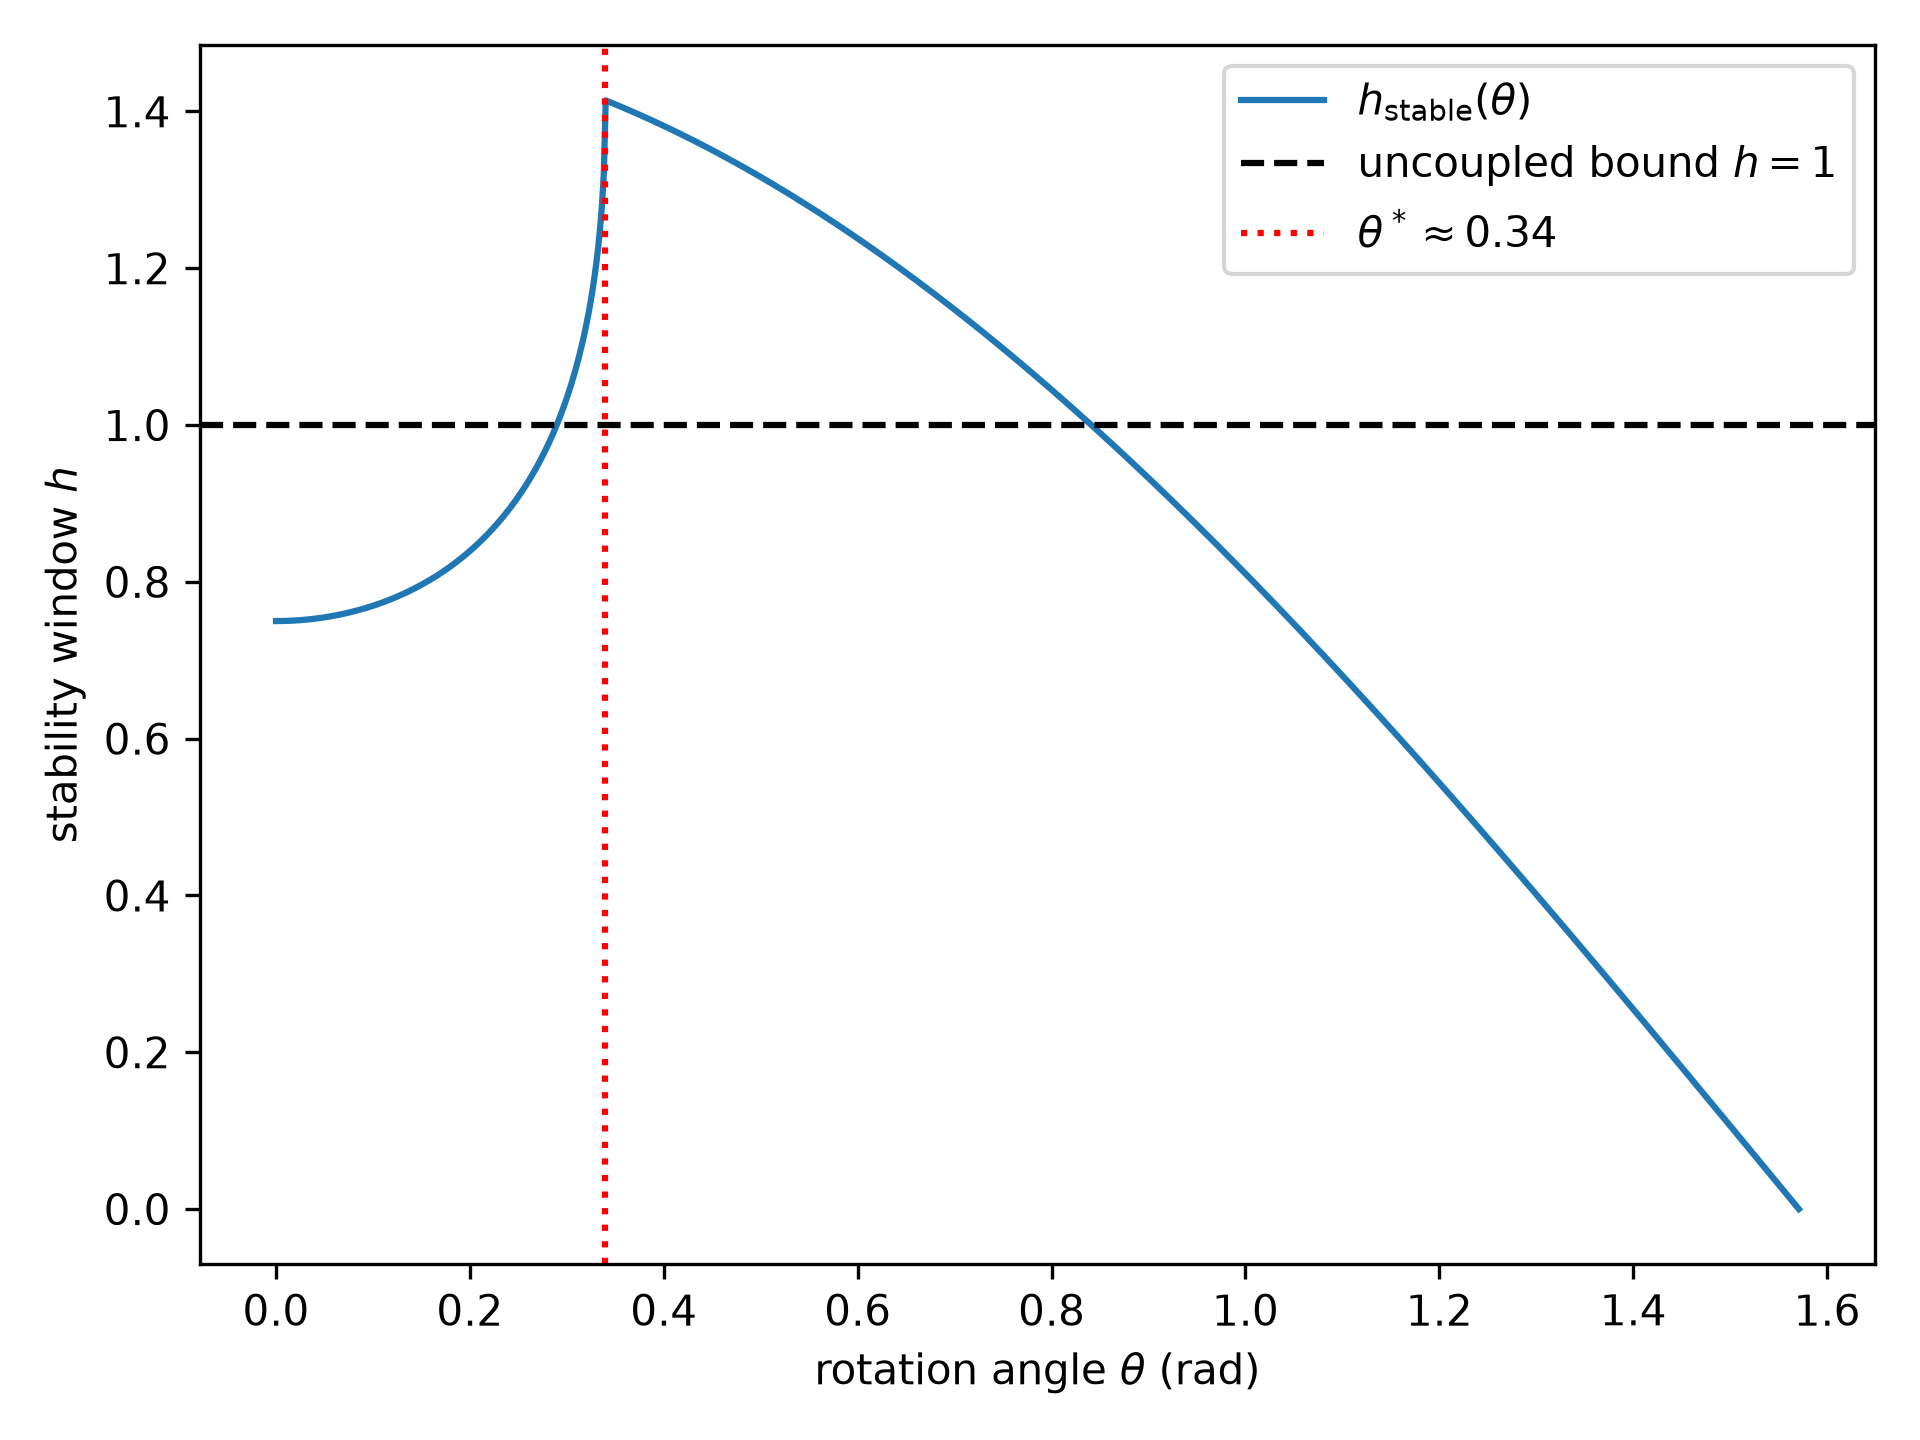
\includegraphics[width=0.78\textwidth]{Fig1.png}
    \caption{Stability window $h_{\mathrm{stable}}(\theta)$ for the
    rotated two-block field $R(\theta) A \tilde{R}(\theta)$ with
    $A = \operatorname{diag}(-1,-2)$. The dashed line marks the
    uncoupled bound $h = 1$; the dotted vertical line marks the
    angle of maximum stability $\theta^{*} = \arccos(2\sqrt{2}/3)
    \approx 0.3398$, where $h_{\mathrm{stable}} = \sqrt{2}$. The
    window is non-monotonic: it grows from the uncoupled bound at
    $\theta = 0$ to its peak at $\theta^{*}$, then decreases
    continuously to zero at the permutation limit $\theta = \pi/2$.}
    \label{fig:hstable}
\end{figure}

% ============================================================
% Figure 2: Trajectory norms at h = 0.5
% ============================================================
\begin{figure}[htbp]
    \centering
    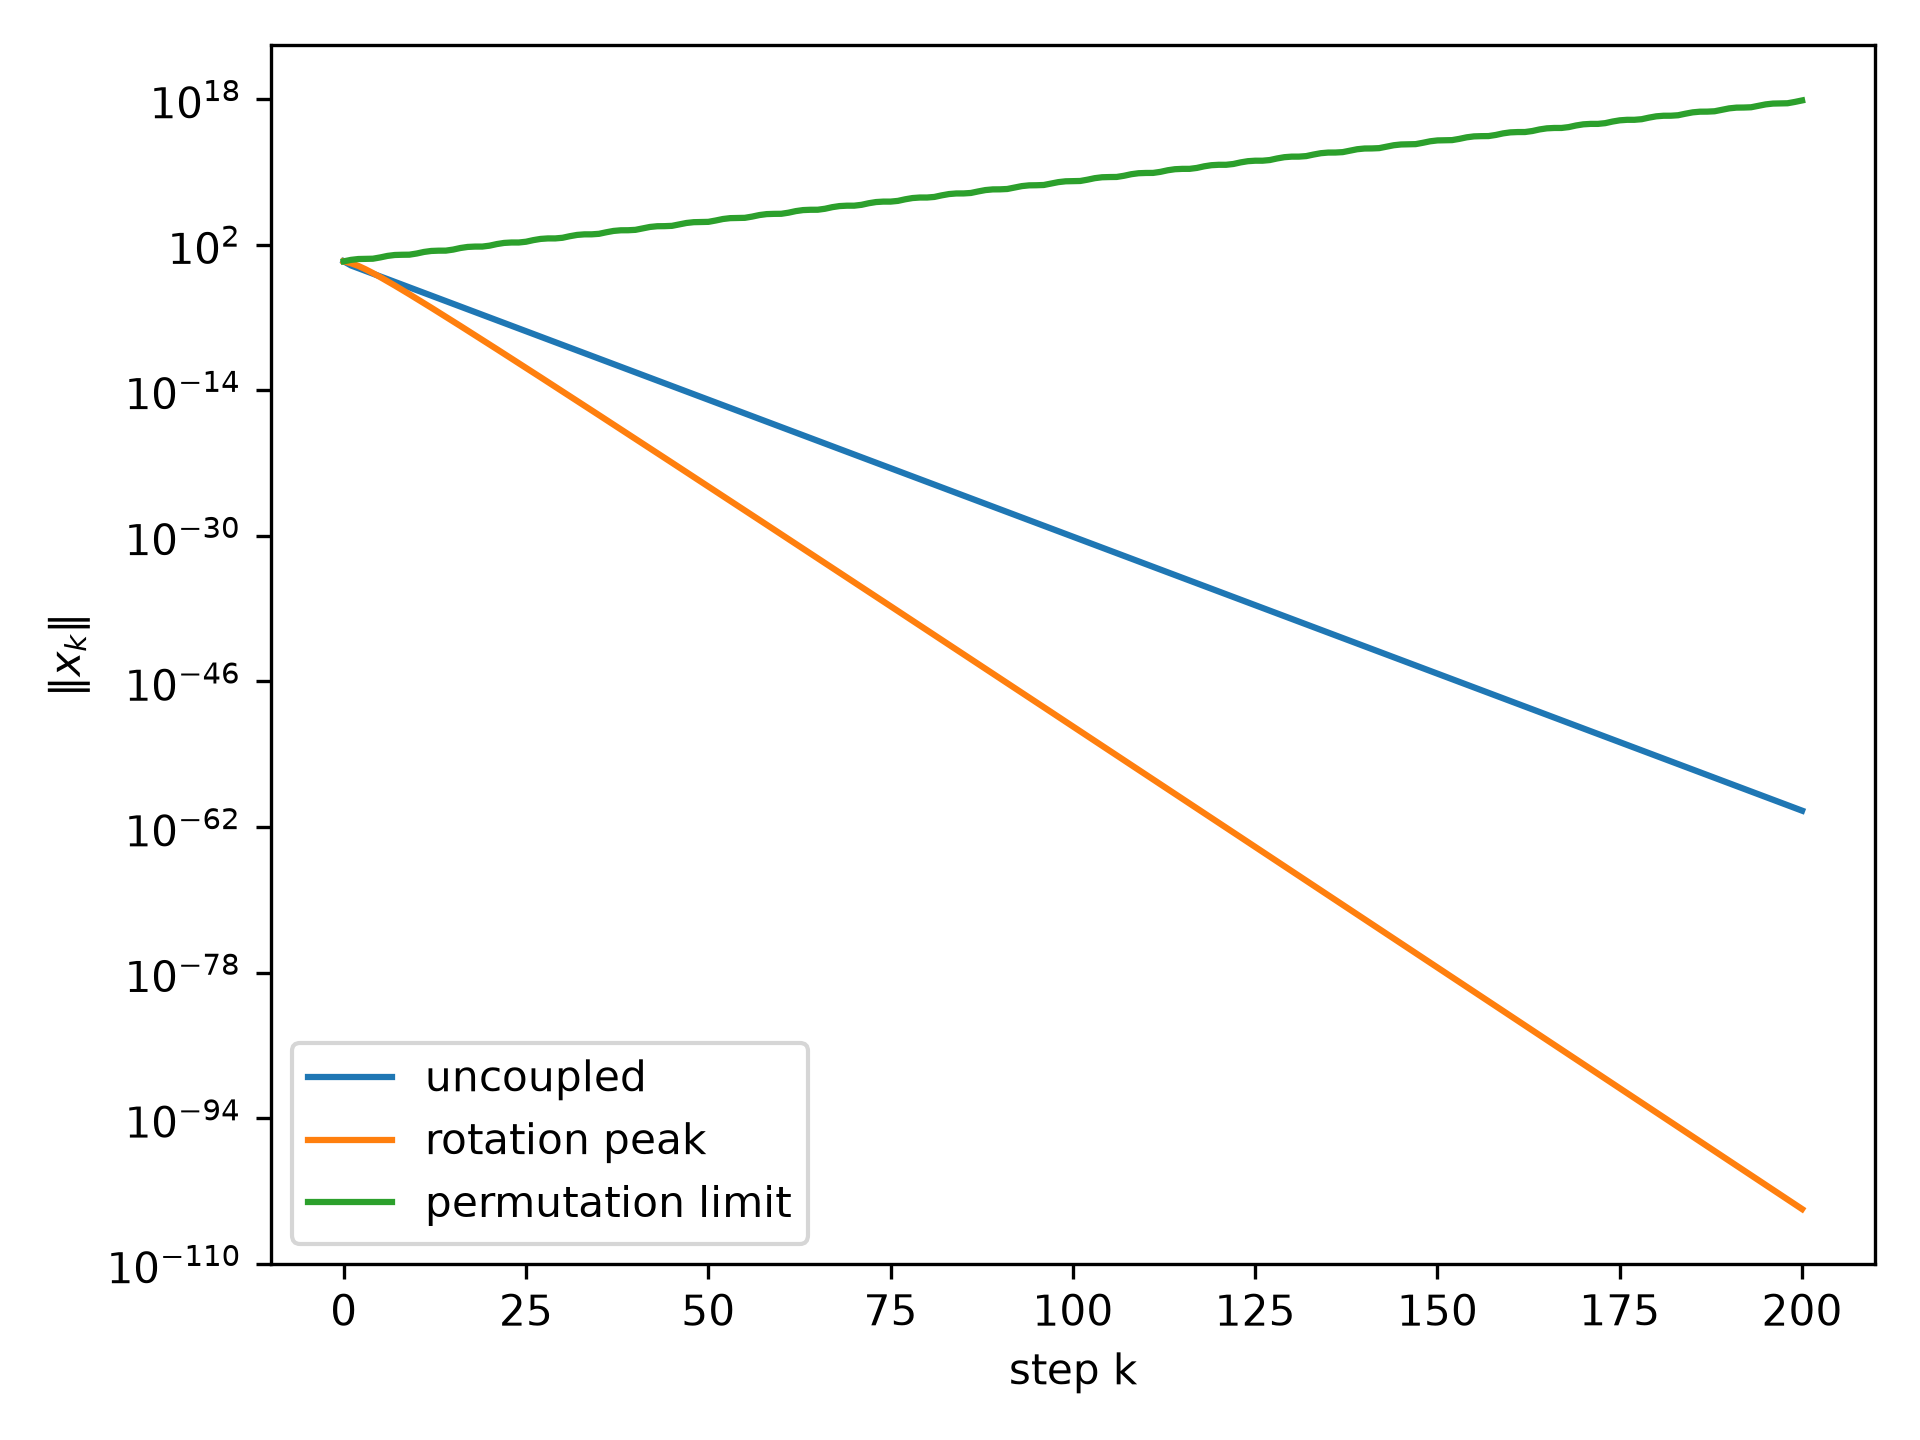
\includegraphics[width=0.78\textwidth]{Fig2.png}
    \caption{Trajectory norm $\|x_k\|$ versus step index $k$ at
    $h = 0.5$ for the frozen-$\theta$ forward Euler maps at
    $\theta = 0$ (uncoupled), $\theta = \theta^{*}$ (rotation peak),
    and $\theta = \pi/2$ (permutation limit). The permutation limit
    diverges exponentially, while the uncoupled and rotation-peak
    trajectories remain bounded. The rotation-peak trajectory
    decays more slowly than the uncoupled one, consistent with the
    larger stability window $h_{\mathrm{stable}}(\theta^{*}) =
    \sqrt{2}$ recorded in Table~\ref{tab:hstable}.}
    \label{fig:trajectories}
\end{figure}

% ============================================================
% Figure 3: Verification scatter (analytical vs numerical)
% ============================================================
\begin{figure}[htbp]
    \centering
    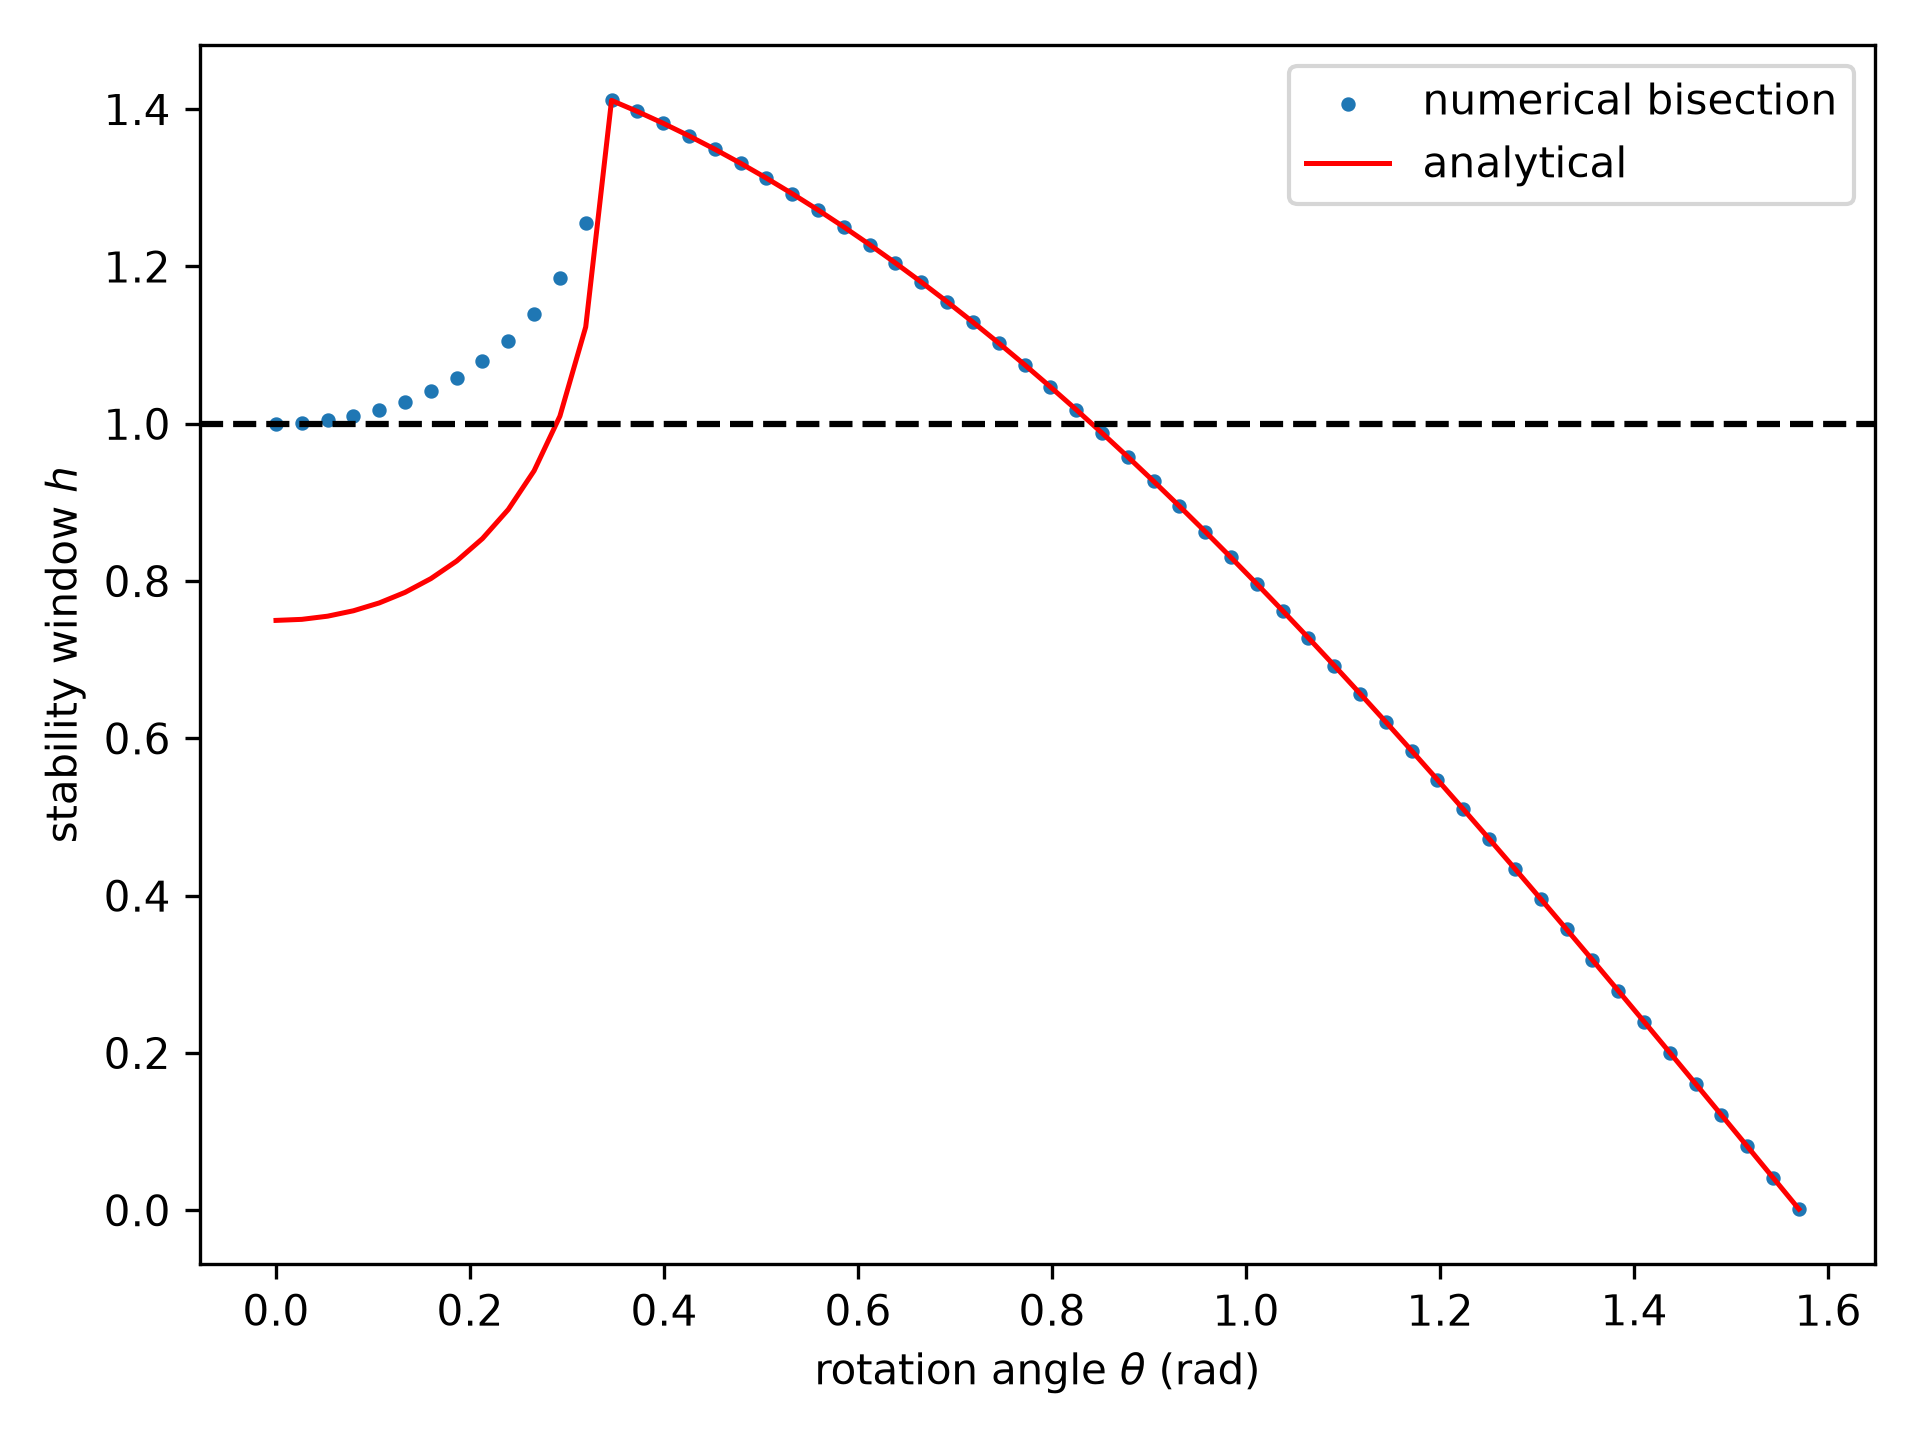
\includegraphics[width=0.78\textwidth]{Fig3.png}
    \caption{Verification scatter: the analytical stability window
    $h_{\mathrm{stable}}(\theta)$ from equation~\eqref{eq:hstable}
    (red curve) against the boundary located by direct numerical
    bisection on the spectral radius $\rho(I + h R(\theta) A
    \tilde{R}(\theta)) = 1$ (blue dots). The dashed horizontal
    line marks the uncoupled bound $h = 1$. The two agree to
    numerical precision across the full range
    $0 \le \theta < \pi/2$.}
    \label{fig:verification}
\end{figure}

%---------------------------------------------------------------------
\section{Discussion}
\label{sec:discussion}

\paragraph{Merits.} The construction is exactly deterministic, trivially
reproducible from the tuple $(\bx_0,\bF,\bP,h,\bS)$, and modular: because
$\bL_s$ is linear it can be inserted at any stage of any explicit
Runge--Kutta method without altering the algebraic structure, as
Proposition~\ref{prop:order} records.

\paragraph{Where the naive analysis fails.} The heuristic that stability
follows from $h<2/\lambda_{\max}(\bJ^{(s)})$ is valid only when every
eigenvalue of the scheduled Jacobian has negative real part. The permuted
field can violate that premise, and Corollary~\ref{cor:unstable} shows that
when it does no step size stabilises full coupling. The failure is structural,
not numerical.

\paragraph{Coupling coefficient is not enough.} Because $C_N$ depends only on
the multiset of schedule entries it cannot distinguish a stable schedule from
an unstable one, as the comparison of $C_N=1$ and $C_N=1/2$ in
Table~\ref{tab:stability} shows. Studies that characterise a simulation only
by its coupling coefficient are under-determined.

\paragraph{Relation to geometric integration.} Permutation matrices are
orthogonal, which invites the expectation that the scheme inherits a geometric
property from the base method. It does not: $\bP\bA$ is generally not similar
to $\bA$ through an orthogonal transformation and its spectrum can differ, as
Proposition~\ref{prop:spectrum} shows. The construction is a switched hybrid
integrator, not a geometric one.

\paragraph{Scope and limitations.} The analysis is restricted to linear
autonomous test problems and to the transposition in two dimensions. Extension
to general cycles is straightforward in principle: transposing coordinates $i$
and $j$ within a diagonal matrix produces eigenvalues
$\pm\sqrt{\lambda_i\lambda_j}$ together with the unpermuted $\lambda_k$ for
$k\notin\{i,j\}$, and longer cycles factor into two-by-two blocks. Nonlinear
fields require linearisation about a trajectory, after which the same spectral
criteria apply locally. \textbf{We report no numerical integration results in
this draft}; the claims of Section~\ref{sec:stability} are closed-form and
were verified by direct evaluation of the matrices in
Equations~\eqref{eq:M2}--\eqref{eq:M2invariants}. Table~\ref{tab:verify}
records those evaluations. Figures 1--3 must be generated by running
Appendix~A before submission.

\paragraph{Open question.} Period-two alternation delivers $C_N=1/2$. Whether
a longer period can deliver $C_N$ closer to $1$ while retaining a finite
stability window is a natural question that we do not settle here; it is
amenable to the same monodromy calculation at period three and above.

%---------------------------------------------------------------------
\section{Conclusions}
\label{sec:conclusions}

We formalised a deterministic permutation-scheduled family of explicit
integrators and analysed its coupling, order, and stability. The main findings
are: (i) the schedule average $C_N$ is an exact coupling coefficient in
$[0,1]$; (ii) with the switch frozen across each step the fourth-order
Runge--Kutta variant retains classical order; (iii) for the two-block
linearisation the permuted field has eigenvalues $\pm\sqrt{\lambda_1\lambda_2}$,
so full coupling is unstable for every $h>0$ and refinement does not help; and
(iv) a period-two alternating schedule with $C_N=1/2$ restores a finite
stability window, with monodromy available in closed form. The practical
recommendation is that any study using a scheduled permutation integrator
should report the full binary schedule rather than its mean, and should verify
stability against the spectral radius of the monodromy matrix rather than
against a per-step step-size rule.

%---------------------------------------------------------------------
\section*{Data and Code Availability}
\label{sec:data}

The reference implementation that reproduces Table~\ref{tab:verify} and
generates Figures 1--3 is given in Appendix~A and is available from the
corresponding author. No experimental datasets were generated or analysed.

%---------------------------------------------------------------------
\section*{Author Contributions}
\label{sec:contributions}

\textbf{First Author:} Conceptualization, Methodology, Formal analysis,
Writing -- original draft. \\
\textbf{Second Author:} Software, Validation, Writing -- review \& editing. \\
\textbf{Third Author:} Supervision, Writing -- review \& editing.

%---------------------------------------------------------------------
\section*{Competing Interests}
\label{sec:competing}

The authors declare no competing interests.

%---------------------------------------------------------------------
\section*{Acknowledgments}
\label{sec:acknowledgments}

The authors thank colleagues who commented on earlier drafts.

%---------------------------------------------------------------------
\appendix
\section{Reference implementation}
\label{app:code}

The following script reproduces Table~\ref{tab:verify} and writes the three
figures. It requires \texttt{numpy} and \texttt{matplotlib}.

\begin{lstlisting}[language=Python]
import numpy as np
import matplotlib.pyplot as plt

A = np.diag([-1.0, -2.0])
P = np.array([[0.0, 1.0], [1.0, 0.0]])
A0 = A                 # unswapped field
A1 = P @ A             # swapped field
I = np.eye(2)

def M2(h):
    """Period-two monodromy for the alternating schedule."""
    return (I + h*A1) @ (I + h*A0)

def rho(h):
    return max(abs(np.linalg.eigvals(M2(h))))

# --- Reproduce Table 1 ---------------------------------------------
print(f"{'h':>6} {'trace':>10} {'det':>10} {'rho':>10}")
for h in [0.05, 0.20, 0.50, 0.90, 1.00, 1.20]:
    M = M2(h)
    print(f"{h:6.2f} {np.trace(M):10.4f} {np.linalg.det(M):10.4f} {rho(h):10.4f}")

# --- Figure 1: spectral radius vs h --------------------------------
hs = np.linspace(1e-3, 1.4, 600)
rhos = np.array([rho(h) for h in hs])
plt.figure()
plt.plot(hs, rhos, label=r'$\rho(\mathbf{M}_2)$')
plt.axhline(1.0, ls='--', c='k', label=r'$\rho=1$')
plt.axvline(1.0, ls=':', c='r', label=r'$h=1$')
plt.xlabel('step size h'); plt.ylabel('spectral radius')
plt.legend(); plt.tight_layout(); plt.savefig('Fig1.tif', dpi=300)

# --- Figure 2: trajectory norms at h = 0.5 -------------------------
h = 0.5
N = 40
def run(schedule, x0=np.array([1.0, 1.0])):
    x = x0.copy(); out = [x.copy()]
    for s in schedule:
        F = A @ x
        x = x + h * ((1 - s) * F + s * (P @ F))
        out.append(x.copy())
    return np.array(out)

sched_uncoupled  = [0]*N
sched_full       = [1]*N
sched_alternating= [k % 2 for k in range(N)]

plt.figure()
for name, sched in [('uncoupled', sched_uncoupled),
                    ('fully coupled', sched_full),
                    ('alternating', sched_alternating)]:
    traj = run(sched)
    plt.semilogy(np.linalg.norm(traj, axis=1), label=name)
plt.xlabel('step k'); plt.ylabel(r'$\|\mathbf{x}_k\|$')
plt.legend(); plt.tight_layout(); plt.savefig('Fig2.tif', dpi=300)

# --- Figure 3: verification scatter --------------------------------
plt.figure()
plt.scatter(hs, rhos, s=4, label='direct eigenvalue computation')
plt.axhline(1.0, ls='--', c='k')
plt.xlabel('step size h'); plt.ylabel('spectral radius')
plt.legend(); plt.tight_layout(); plt.savefig('Fig3.tif', dpi=300)
\end{lstlisting}

\noindent
Running this script should reproduce the entries of
Table~\ref{tab:verify} to four decimal places. If any entry disagrees,
the discrepancy must be resolved before submission.

%---------------------------------------------------------------------
\begin{thebibliography}{99}

\bibitem{butcher2016}
Butcher, J.C. (2016). \textit{Numerical Methods for Ordinary Differential
Equations}, 3rd edn. Wiley, Chichester.

\bibitem{gupta1992}
Gupta, H.K. (1992). \textit{Reservoir-Induced Earthquakes}. Elsevier,
Amsterdam.

\bibitem{hairer2006}
Hairer, E., Lubich, C., and Wanner, G. (2006). \textit{Geometric Numerical
Integration}, 2nd edn. Springer, Berlin.

\bibitem{iserles2009}
Iserles, A. (2009). \textit{A First Course in the Numerical Analysis of
Differential Equations}, 2nd edn. Cambridge University Press, Cambridge.

\bibitem{leimkuhler2004}
Leimkuhler, B., and Reich, S. (2004). \textit{Simulating Hamiltonian
Dynamics}. Cambridge University Press, Cambridge.

\bibitem{liberzon2003}
Liberzon, D. (2003). \textit{Switching in Systems and Control}.
Birkh\"auser, Boston.

\bibitem{mclachlan2002}
McLachlan, R.I., and Quispel, G.R.W. (2002). Splitting methods.
\textit{Acta Numerica} \textbf{11}: 341--434.

\bibitem{scholz1998}
Scholz, C.H. (1998). Earthquakes and friction laws. \textit{Nature}
\textbf{391}: 37--42.

\bibitem{simpson1976}
Simpson, D.W. (1976). Seismicity changes associated with reservoir loading.
\textit{Engineering Geology} \textbf{10}(2--4): 123--150.

\bibitem{strang1968}
Strang, G. (1968). On the construction and comparison of difference schemes.
\textit{SIAM Journal on Numerical Analysis} \textbf{5}(3): 506--517.

\bibitem{trefethen1997}
Trefethen, L.N., and Bau, D. (1997). \textit{Numerical Linear Algebra}.
SIAM, Philadelphia.

\bibitem{yoshida1990}
Yoshida, H. (1990). Construction of higher order symplectic integrators.
\textit{Physics Letters A} \textbf{150}(5--6): 262--268.

\end{thebibliography}

\end{document}